\documentclass[12pt]{article} % use larger type; default would be 10pt

\usepackage[polish]{babel}
\usepackage[utf8]{inputenc}
\usepackage{t1enc}

\usepackage{amsfonts}
\usepackage{amsmath}

\usepackage{hyperref}
\usepackage{graphicx}

\addtolength{\textwidth}{3cm}
\addtolength{\textheight}{5.5cm}
\addtolength{\voffset}{-2.5cm}
\addtolength{\hoffset}{-1cm}

\renewcommand\baselinestretch{1.1}


\DeclareMathOperator{\Q}{\mathbb{Q}} 
\DeclareMathAlphabet{\mathpzc}{OT1}{pzc}{m}{it}

\def\R{\mathbb{R}} 
\def\N{\mathbb{N}}
\def\Z{\mathbb{Z}}

\def\CC{\mathcal{C}}
\def\FF{\mathcal{F}} 
\def\MM{\mathcal{M}} 
\def\NN{\mathcal{N}} 

\newcommand{\nnatural}{\mathbb{N}}
\newcommand{\rational}{\mathbb{Q}}
\newcommand{\real}{\mathbb{R}}
\newcommand{\integers}{\mathbb{Z}}
\newcommand{\complex}{\mathbb{C}}

\newcounter{zad}
\def\numzad{\smallskip\noindent\refstepcounter{zad}{\bf Zadanie \thezad.} }
\pagestyle{empty}

\date{}

\begin{document}

\bigskip
\centerline{\large{\bf{Zadania z kombinatoryki (seria nr 1)}}}
\bigskip

\numzad
  W wagonie kolejowym jest $8$ ponumerowanych miejsc w dwóch rzędach po $4$ miejsca.  Do pustego wagonu
weszło $5$ osób: $3$ panie i $2$ panów. Panie zajęły miejsca w jednym rzędzie a panowie usiedli 
w drugim. Oblicz na ile sposobów osoby te mogły zająć miejsca tak, aby vis-\`{a}-vis
każdego z panów siedziała pani.

\numzad
  Uzasadnij kombinatorycznie, że $\forall_{n,k \in \nnatural, k \leq n} k {n \choose k} = n {n -1 \choose k - 1}$. 


\numzad 
  Podaj definicję liczb Catalana i oblicz $C_5$.

\medskip 

{\tt Wskazówka: można na przykład za pomocą wzoru rekurencyjnego: każda liczba Catalana to wektor poprzednich liczb
Catalana pomnożony skalarnie przez ten sam wektor tylko zapisany w odwrotnej kolejności, szczegóły do wyszukania w notatkach/sieci etc.}

\numzad 
  Podaj definicję liczb Bella i oblicz $B_5$.

\medskip 

{\tt Wskazówka: można na przykład za pomocą wzoru rekurencyjnego:
  $B_{n+1} = \sum_{j = 0}^n {n \choose j} B_j$
szczegóły do wyszukania w notatkach/sieci etc.}

\numzad
  Dana jest rodzina $\mathcal{A} = (A_1, A_2, \ldots, A_{10})$, gdzie
$A_1 = \lbrace 1,3,5 \rbrace$,
$A_2 = \lbrace 2,4,6 \rbrace$,
$A_3 = \lbrace 1,3,5 \rbrace$,
$A_4 = \lbrace 3,5 \rbrace$,
$A_5 = \lbrace 4,5 \rbrace$,
$A_6 = \lbrace 2,4,5,6,7 \rbrace$,
$A_7 = \lbrace 2,3,4,5,6 \rbrace$,
$A_8 = \lbrace 7,8 \rbrace$,
$A_9 = \lbrace 5,6,7,8,9 \rbrace$,
$A_{10} = \lbrace 1,3,8,9,10 \rbrace$.
Czy ta rodzina posiada transwersalę ({\tt Inna nazwa: system rozłącznych reprezentantów - SDR,
proponuję odnośnie definicji prześledzić to: \url{https://pl.wikipedia.org/wiki/Transwersala}})?
Odpowiedź uzasadnij.

\medskip
{
\tt
  To jest zadanie na tak zwane twierdzenie Halla. Skanowałem swego czasu odpowiednie
notatki, ale przypomnę że twierdzenie Halla podaje warunek konieczny i dostateczny
na istnienie transwersali, proponuję koniecznie zapoznać się z tymi artykułami:
\url{https://pl.wikipedia.org/wiki/Twierdzenie_o_kojarzeniu_ma%C5%82%C5%BCe%C5%84stw}
- ale wersja o transwersalach - wersja o grafach w naszym kontekście nie jest 
potrzebna. Tam jest ów warunek Halla i po prostu trzeba z niego skorzystać w tym zadaniu.

\begin{figure}[ht!]
\centering
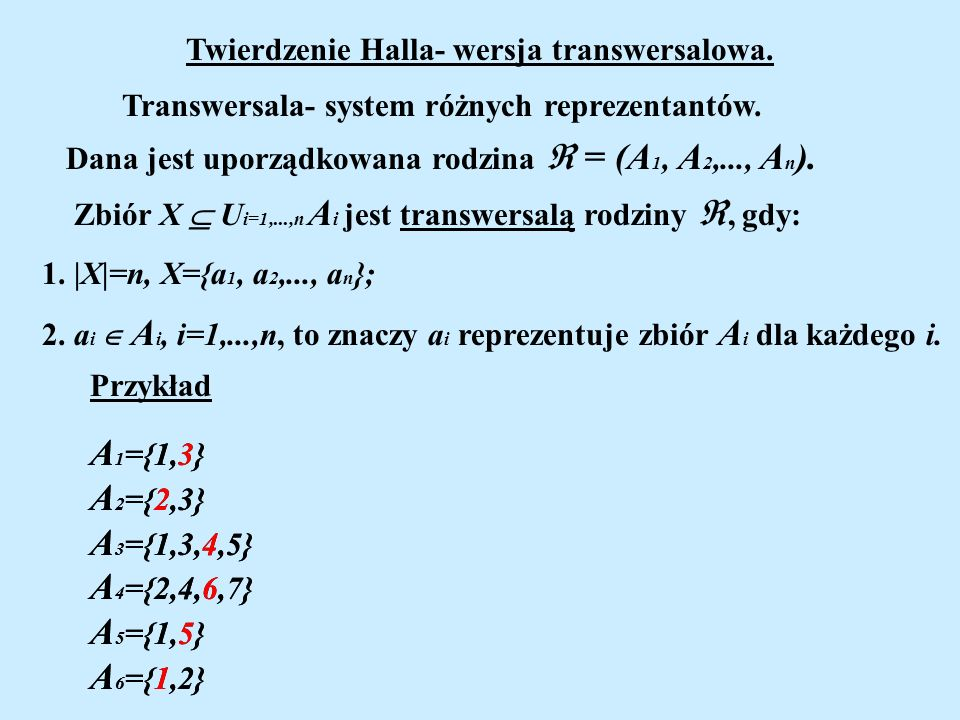
\includegraphics[width=90mm]{transwersala_przyklad.jpg}
\caption{Przykład na transwersalę (skopiowany z Sieci)}
\end{figure}
}

\numzad
  Na ile sposobów można rozmieścić $128$ osób w $7$ ponumerowanych wagonach
pociągu? Na ile sposobów możemy rozmieścić $128$ osób w $7$ 
{\tt (też oczywiście ponumerowanych)} wagonach tak, aby żaden wagon
nie był pusty?

\numzad 
  Przed kasą muzeum ustawiła się $100$-osobowa kolejka. Bilety są po $10$ złotych.
połowa z tych osób ma banknot $10$ złotowy, druga połowa zaś
tylko banknot $20$ złotowy. Jakie jest prawdopodobieństwo, że żadna z osób nie
będzie zmuszona czekać na wydanie reszty?

{\tt To jest klasyczne zadanie na tak zwane ,,liczby Catalana'' - i wzór na nie 
($c_n = {1 \over n + 1} {2n \choose n}$) . Tutaj: 
\url{http://liczbycatalana.blogspot.com/} jest cały blog (sic!!!) o rzeczonych liczbach.
Ale akurat wzmianki o tym zadaniu tam nie ma, proponuję poszperać w Sieci lub
w moich skanach.
}

\end{document}
